% Teilaufgabe 7

\newpage
\section{Spektren der verwendeten Lampen dieses Versuches}
\label{sec:spekternLampen}

\begin{enumerate}
	\item Halogenlampe
	\begin{center}
		\captionsetup{type=figure}
		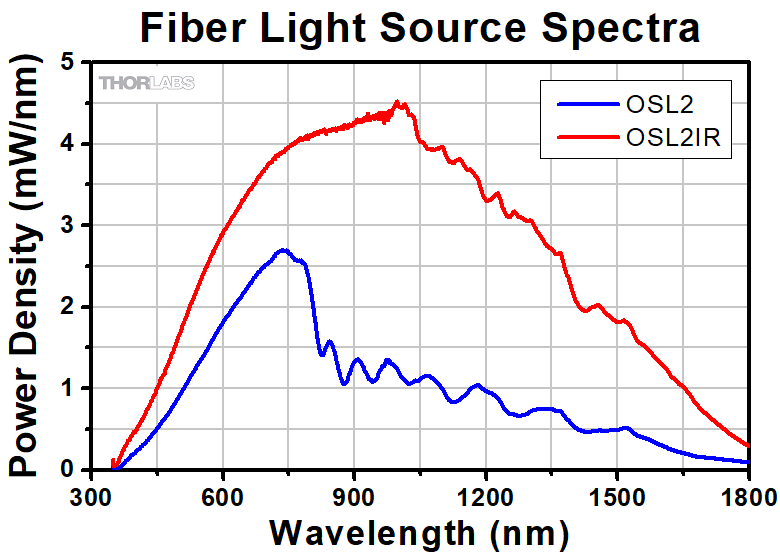
\includegraphics[width=0.75\textwidth]{Spektrum-Halogen.png}
		\captionof{figure}{Spektrum einer Halogenlampe. \cite{halogenlamp}}
		\label{fig:halogen}
	\end{center}
	\item Deuteriumlampe
	\begin{center}
		\captionsetup{type=figure}
		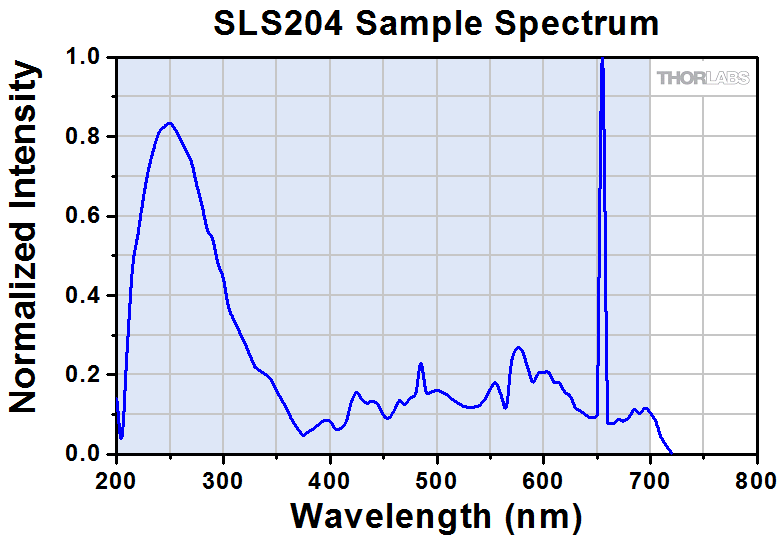
\includegraphics[width=0.75\textwidth]{Spektrum-Deuterium.png}
		\captionof{figure}{Spektrum einer Deuteriumlampe. \cite{deuteriumlamp}}
		\label{fig:deuterium}
	\end{center}
\end{enumerate}
